%%%%%%%%%%%%%%%%%%%%%%%%%%%%%%%%%%%%%%%%%%%%%%%%%%%%%%%%%%%%%%%%%%%%%%%%%%%%%%%%
% Power
%%%%%%%%%%%%%%%%%%%%%%%%%%%%%%%%%%%%%%%%%%%%%%%%%%%%%%%%%%%%%%%%%%%%%%%%%%%%%%%%
\chapter{Power} \label{Power}
\vspace{-10ex}\mPo{syml}\vskip 8ex

%%%%%%%%%%%%%%%%%%%%%%%%%%%%%%%%%%%%%%%%%%%%%%%%%%%%%%%%%%%%%%%%%%%%%%%%%%%%%%%%
% Introduction
%%%%%%%%%%%%%%%%%%%%%%%%%%%%%%%%%%%%%%%%%%%%%%%%%%%%%%%%%%%%%%%%%%%%%%%%%%%%%%%%
\section{Introduction}

In order to prolong battery charge, the \cDi{f} and \cLi{f} can, depending on
mode, turn \sScOf{f} or \sScDi{f} after a configurable period of inactivity.
The device can also enter a low power \sPoSl{f} state to further reduce power
consumption and auto-stop the \mAu{f} if it isn't being used.  See
\hyperref[Power Settings]{\mPS{f}} for configuration.

%%%%%%%%%%%%%%%%%%%%%%%%%%%%%%%%%%%%%%%%%%%%%%%%%%%%%%%%%%%%%%%%%%%%%%%%%%%%%%%%
% Wake
%%%%%%%%%%%%%%%%%%%%%%%%%%%%%%%%%%%%%%%%%%%%%%%%%%%%%%%%%%%%%%%%%%%%%%%%%%%%%%%%
\section{Wake} \label{Power - Wake} \sPoAw{syml}

This is the normal operating state and also is the most power consumptive.
The \cDi{f} is \sScOn{f} and the \cLi{f} window is potentially lit, both at the
brightness level as determined by the \cBr{f}.

\par\medskip

Any kind of interaction with the controls of the device will either wake it or
keep it awake.

\begin{itemize}
  \item \aTo{f} the \dTo{f} of the device.\footnote{ Assumes touch capability
    has been enabled via \hyperref[Touch Settings]{\mTS{ss}}.}.
  \item \aTu{f} the \cRs{f}.
  \item \aTu{f} or \aPr{f} the \cEs{f}.
  \item \aTu{f} the \cBr{f}.
  \item \aPr{f} the \cPl{f}, \cNe{f} or \cPr{f} push-buttons.
\end{itemize}

\info{If in the \sPoSl{f} state, neither the \cNe{f} nor the \cPr{f}
push-buttons can wake it though they will keep it from going into a \sPoSl{f}
state.}

\par\medskip

\info{When in \mTS{f} mode and the power state is \sPoNa{f}, \aTo{f} will not
wake it.}

\ers{1}
\begin{longtabu} { X[1,c,m] | X[2,c,m] }
  \thrule
  \thbi{Action} & \thbi{Control} \\ \mrule

  \multirow{3}{*}{\aTu{n}}
    & \hyperref[Operation - Selector Dial]{\cRs{f}} \\
    & \hyperref[Operation - Settings Knob]{\cEs{f}} \\
    & \hyperref[Brightness Knob]{\cBr{f}} \\ \drule{2}

  \multirow{4}{*}{\aPr{n}}
    & \hyperref[Operation - Settings Knob]{\cEs{f}} \\
    & \hyperref[Audio - Play|Pause|Stop]{\cPl{f}} \\
    & \hyperref[Audio - Next]{\cNe{f}}\footnote{ The \cNe{ss} push-button
      will \textit{not} wake if sleeping.} \\
    & \hyperref[Audio - Previous]{\cPr{f}}\footnote{ The \cPr{ss} push-button
      will \textit{not} wake if sleeping.} \\ \drule{2}

  \aTo{n} & \hyperref[Operation - Touch Sensor]{\cTS{f}}\footnote{ Touch
    will \textit{not} wake when napping and in \mTS{ss} mode.} \\

  \bhrule
\caption{Power - Waking Control Actions}
\end{longtabu}

Additionally, the \mAl{f} will wake the device from any power state. It will
also keep it from entering a \sPoSl{f} state as long as it is in the \sAlWa{f}
state and actively alerting or playing music or \sAlIP{f} and the wakeup source
is the \mAu{f}.

%%%%%%%%%%%%%%%%%%%%%%%%%%%%%%%%%%%%%%%%%%%%%%%%%%%%%%%%%%%%%%%%%%%%%%%%%%%%%%%%
% Nap
%%%%%%%%%%%%%%%%%%%%%%%%%%%%%%%%%%%%%%%%%%%%%%%%%%%%%%%%%%%%%%%%%%%%%%%%%%%%%%%%
\section{Nap} \label{Power - Nap} \sPoNa{syml}

The device will \sPoNa{f} if a nap timer has been enabled via
\hyperref[Power Settings]{\mPS{f}} and the following conditions are met:

\begin{itemize}
  \item You are \textit{not} actively using the device, i.e. not interacting
    with it or fiddling with the controls.
  \item The nap timer is enabled and the configured nap timer has elapsed.
\end{itemize}

The nap timer is started from the last time the device was interacted with. For
example, if the \cEs{f} was just turned, the timer will start from that point.
As long as you are interacting with the device, it will \textit{not} \sPoNa{f}.

\par\medskip

The screens will either \sDim{f} or turn \sOff{f} depending on the current mode
and state.

\begin{table}[H]
  \begin{tabu} { X[1,c,m] | X[1,c,m] | X[1,c,m] }
  \thrule
  \thbi{Mode} & \thbi{State} & \thbi{Screens} \\ \mrule

  \hyperref[Clock]{\mCl{s}} & \state{f}{ANY} & \sDim{sym} \\ \mrule

  \multirow{3}{*}[-2.0mm]{\hyperref[Timer]{\mTi{s}}}
    & \sTiRu{f} & \multirow{2}{*}{\sDim{sym}} \\
    & \sTiAl{f} & \\ \dcrule{2}{3}
    & \fontTGA{ss}{ALL OTHER STATES} & \sOff{sym} \\ \mrule

  \multirow{5}{*}[-2.0mm]{\hyperref[Touch Settings]{\mTS{s}}}
    & \sTSBR{f} & \multirow{4}{*}{\sDim{sym}} \\
    & \sTSTR{f} & \\
    & \sTSRT{f} & \\
    & \sTSTA{f} & \\ \dcrule{2}{3}
    & \fontTGA{ss}{ALL OTHER STATES} & \sOff{sym} \\ \mrule

  \fontTGA{f}{ALL OTHER MODES} & \state{f}{ANY} & \sOff{sym} \\

  \bhrule
  \end{tabu}
\caption{Power - Nap Action per Mode}
\end{table}

%%%%%%%%%%%%%%%%%%%%%%%%%%%%%%%%%%%%%%%%%%%%%%%%%%%%%%%%%%%%%%%%%%%%%%%%%%%%%%%%
% Sleep
%%%%%%%%%%%%%%%%%%%%%%%%%%%%%%%%%%%%%%%%%%%%%%%%%%%%%%%%%%%%%%%%%%%%%%%%%%%%%%%%
\section{Sleep} \label{Power - Sleep} \sPoSl{syml}

When the device sleeps, the screens will turn \sOff{f}, the \mAu{f} will go into
the \sAuSt{f} state and all processing stops affording more power savings over
\sPoNa{f}.

\par\medskip

The device will \sPoSl{f} if a sleep timer has been enabled via
\hyperref[Power Settings]{\mPS{f}} and \textit{all} of the following conditions
are met:

\begin{itemize}
  \item You are not actively using the device, i.e. not interacting with it or
    fiddling with the controls.
  \item The \mAu{f} is \textit{not} in the \sAuPl{f} state.
  \item The \mAl{f} is \textit{not} in the \sAlWa{f} state.
  \item The \mAl{f} is \textit{not} \sAlIP{f} when the wakeup source is \mAu{f}.
  \item The current state in the current mode allows \sPoSl{f}.
  \item The sleep timer is enabled and the configured sleep timer has elapsed.
\end{itemize}

The sleep timer is started from the last time the device was interacted with.
For example, if the \cNe{f} push-button is being pressed, the timer will start
from that point.  As long as you are interacting with the device, it will
\textit{not} \sPoSl{f}.

\par\medskip

The timer is also restarted if the \mAu{f} is playing or the \mAl{f} is
alerting.  As long as the \mAu{f} is in the \sAuPl{f} state or the \mAl{f} is in
the \sAlWa{f} state, the device will \textit{not} \sPoSl{f}.

\par\medskip

Additionally, if the \mAl{f} is \sAlIP{f}, i.e. in the \sAlWa{f} or \sAlSn{f}
states \textit{and} the wakeup source is the \mAu{f}, the device will
\textit{not} \sPoSl{f}.  When the wakeup source is the \mAu{f} and the \mAl{f}
is snoozed, the \mAu{f} is \textit{not} stopped, but paused.  Since the
\sPoSl{f} state will \sAuSt{f} the \mAu{f}, the device will \textit{not}
\sPoSl{f} in this situation.

\par\medskip

\info{Though the \cNe{f} and \cPr{f} push-buttons can keep the device from
entering a \sPoSl{f} state, they can \textit{not} wake the device from
\sPoSl{f}.}

\par\medskip

Some modes can be in states that do \textit{not} allow the device to enter a
\sPoSl{f} state.  The following table shows which modes and states can and
cannot enter a \sPoSl{f} state.

\begin{table}[H]
  \begin{tabu} { X[1,c,m] | X[1,c,m] | X[1,c,m] }
  \thrule
  \thbi{Mode} & \thbi{State} & \thbi{Can Sleep?} \\ \mrule

  \multirow{3}{*}[-2.0mm]{\hyperref[Timer]{\mTi{s}}}
    & \sTiRu{f} & \multirow{2}{*}{\fontTGA{f}{NO}} \\
    & \sTiAl{f} & \\ \dcrule{2}{3}
    & \fontTGA{ss}{ALL OTHER STATES} & \fontTGA{f}{YES} \\ \mrule

  \multirow{5}{*}[-2.0mm]{\hyperref[Touch Settings]{\mTS{s}}}
    & \sTSBR{f} & \multirow{4}{*}{\fontTGA{f}{NO}} \\
    & \sTSTR{f} & \\
    & \sTSRT{f} & \\
    & \sTSTA{f} & \\ \dcrule{2}{3}
    & \fontTGA{ss}{ALL OTHER STATES} & \fontTGA{f}{YES} \\ \mrule

  \fontTGA{f}{ALL OTHER MODES} & \state{f}{ANY} & \fontTGA{f}{YES} \\
  \bhrule
  \end{tabu}
\caption{Power - Sleep per Mode \& State}
\end{table}

\pagebreak

Any mode or state that can not \sPoSl{f} will instead \sPoNa{f} and \sDim{f}
the screens.

\begin{table}[H]
  \begin{tabu} { X[1,c,m] | X[1,c,m] | X[1,c,m] }
  \thrule
  \thbi{Mode} & \thbi{State} & \thbi{Action} \\ \mrule

  \multirow{2}{*}[-1.0mm]{\hyperref[Timer]{\mTi{s}}}
    & \sTiRu{f} & \multirow{6}{*}{\sPoSl{f} $\longrightarrow$ \sPoNa{f}} \\
    & \sTiAl{f} & \\ \dcrule{1}{2}

  \multirow{4}{*}[-1.5mm]{\hyperref[Touch Settings]{\mTS{s}}}
    & \sTSBR{f} & \\
    & \sTSTR{f} & \\
    & \sTSRT{f} & \\
    & \sTSTA{f} & \\

  \bhrule
  \end{tabu}
\caption{Power - Sleep to Nap}
\end{table}

%%%%%%%%%%%%%%%%%%%%%%%%%%%%%%%%%%%%%%%%%%%%%%%%%%%%%%%%%%%%%%%%%%%%%%%%%%%%%%%%
% Sleep - Touch Sleep
%%%%%%%%%%%%%%%%%%%%%%%%%%%%%%%%%%%%%%%%%%%%%%%%%%%%%%%%%%%%%%%%%%%%%%%%%%%%%%%%
\subsection{Touch Sleep} \label{Power - Touch}

The device can be \textit{forced} into a \sPoSl{f} state by
\textit{continuously} touching the \cTo{f} of the device for a configurable
amount of time set via \hyperref[Power Settings]{\mPS{f}}.  Though the sleep
timer is reset when touched, it is irrelevant if this touch time is exceeded.
Since the device is forced into a \sPoSl{f} state, the \mAu{f} will be
\textit{forced} into the \sAuSt{f} state.

\info{For touch induced sleep to work, \aTo{f} must be enabled via
\hyperref[Touch Settings]{\mTS{f}} and the palm of your hand or
most of your fingers must lay on \cTo{f} of the enclosure.}

%%%%%%%%%%%%%%%%%%%%%%%%%%%%%%%%%%%%%%%%%%%%%%%%%%%%%%%%%%%%%%%%%%%%%%%%%%%%%%%%
% Audio Auto-Stop
%%%%%%%%%%%%%%%%%%%%%%%%%%%%%%%%%%%%%%%%%%%%%%%%%%%%%%%%%%%%%%%%%%%%%%%%%%%%%%%%
\section{Audio Auto-Stop} \label{Power - Stop}

The \mAu{f} component will automatically \sAuSt{f} if a stop timer has been
enabled via \hyperref[Power Settings]{\mPS{f}} and \textit{all} of the
following conditions are met:

\begin{itemize}
  \item You are not actively using the device, i.e. not interacting with it or
    fiddling with the controls.
  \item The \mAu{f} is in the \sAuPa{f} state.
  \item The \mAl{f} is \textit{not} \sAlIP{f} \textit{or} is \textit{not} using
    the \mAu{f} as the wakeup source.
  \item The stop timer is enabled and the configured stop timer has elapsed.
\end{itemize}

The stop timer is started from the last time the device was interacted with.
For example, if the \cBr{f} was just turned, the timer will start from that
point.  As long as you are interacting with the device, the \mAu{f} will
\textit{not} be auto-stopped.

\par\medskip

The timer is also restarted if the \mAu{f} is playing or the \mAl{f} is
\sAlIP{f}, i.e. in the \sAlWa{f} or \sAlSn{f} states \textit{and}
the wakeup source is the \mAu{f}.  As long as these conditions are true,
the device will \textit{not} auto-stop the \mAu{f}.

%%%%%%%%%%%%%%%%%%%%%%%%%%%%%%%%%%%%%%%%%%%%%%%%%%%%%%%%%%%%%%%%%%%%%%%%%%%%%%%%
% State Diagram
%%%%%%%%%%%%%%%%%%%%%%%%%%%%%%%%%%%%%%%%%%%%%%%%%%%%%%%%%%%%%%%%%%%%%%%%%%%%%%%%
\section{State Diagram}

\begin{figure}[H]
\centering
  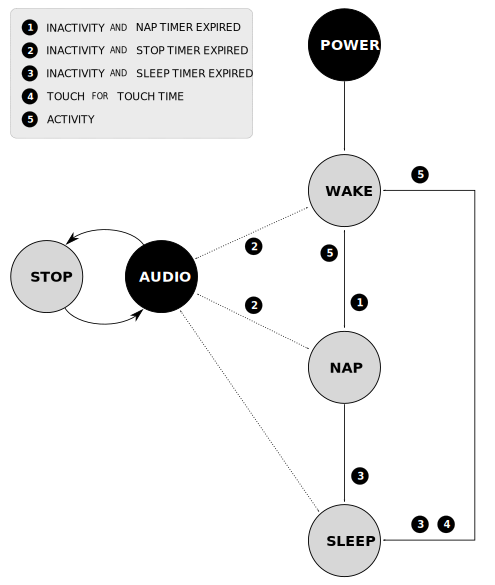
\includegraphics{images/power_state_diagram.png}
\caption{Power - State Diagram}
\end{figure}
